\section{Results}
\subsection{Model Integration and Completion}
\label{sec:integration}
Figure~\ref{fig:integration} compares direct model-selected placement with cached interpretation and numerical scheduling. Under updated contracts, the respective completion counts are 9,729 versus 21,507 for Jev, 15,639 versus 20,355 for DeepSeek, and 13,130 versus 19,537 for Gemini, each out of 22,500 requests. The structured-input reference completes 22,312. All three models interpret the contract profiles correctly in this block. The performance difference therefore involves how those contracts are converted into a placement and when the placement takes effect.

\begin{figure}[t]
\centering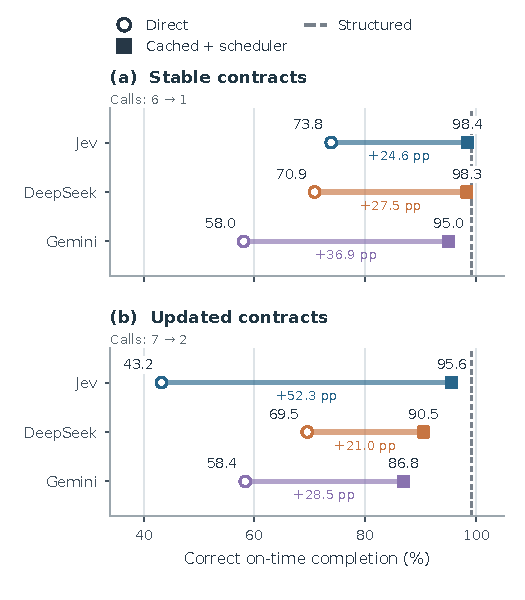
\includegraphics[width=\columnwidth]{figures/integration.pdf}
\caption{Integration comparison with modeled edge execution. Endpoint labels give completion percentages for direct placement (open circles) and cached interpretation with numerical scheduling (squares); connector labels give percentage-point gains. Dashed lines show the structured-input reference. Call counts compare direct and cached configurations. Each mark is one trajectory with 22,500 requests; scheduling responsibility and semantic reuse change together.}
\label{fig:integration}
\end{figure}

The numerical scheduler jointly accounts for offered load, worker capacity, and transport delay relative to the serving cell. A placement can obey all location permissions yet concentrate enough work at one worker to delay many requests. Separating these resource decisions from semantic interpretation substantially improves completion for each tested model. For Jev, the updated-condition completion fraction increases from 43.24\% to 95.59\%.

Reuse also reduces interpretation frequency. Stable contracts require six model calls in direct orchestration and one in the cached configuration. Updated contracts require seven and two, respectively. Each cached trajectory has five hits, while the scheduler continues to reconsider placement using current observations. We use this integration in the remaining comparisons: interpret new contracts once and schedule against current numerical state.

\subsection{Correct Interpretation with Lower Response Time}
\label{sec:latency}
\begin{figure*}[t]
\centering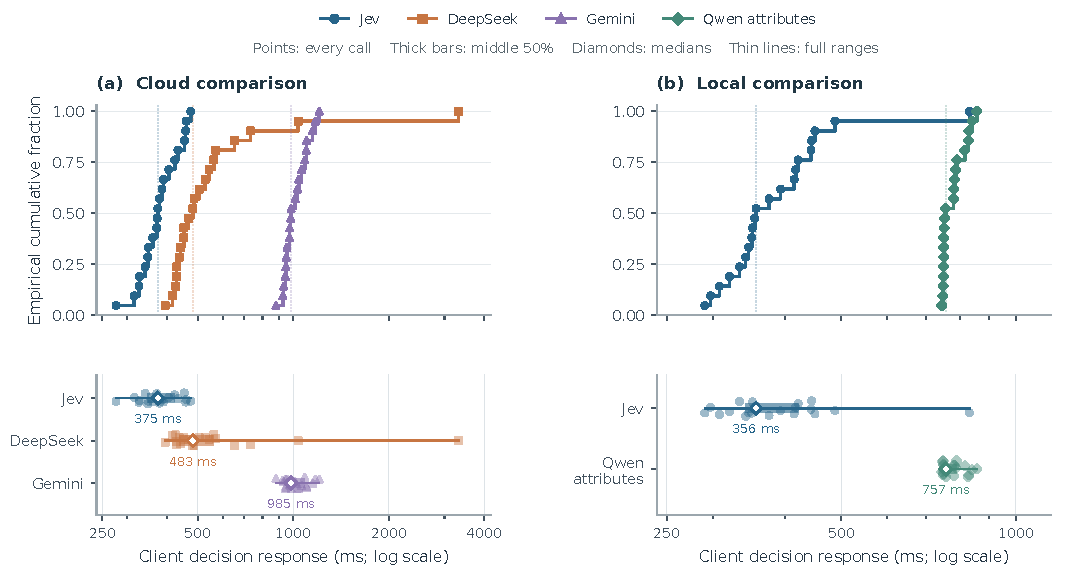
\includegraphics[width=\textwidth]{figures/decision-distributions.pdf}
\caption{Measured decision-response distributions. Upper plots show empirical cumulative fractions for all 21 calls per model. Lower strips retain every call, with deterministic vertical offsets for visibility; thick bars span the 25th--75th percentiles, diamonds and labels give medians, and thin lines show full ranges. The cloud and local blocks have separate contemporaneous Jev measurements. Logarithmic axes retain the complete ranges, including DeepSeek's 3.315-second response. Quantiles describe calls, not confidence intervals.}
\label{fig:latencies}
\end{figure*}
\begin{table}[t]
\centering
\caption{Cloud comparison. Response cells give the median and [25th, 75th] percentiles in milliseconds over 21 calls per model. Contract accuracy uses 63 checks; completion is the mean over nine updated-contract trajectories.}
\label{tab:cloud}
\footnotesize\setlength{\tabcolsep}{4pt}\renewcommand{\arraystretch}{1.16}
\begin{tabular}{@{}lrrr@{}}\toprule
& \multicolumn{2}{c}{Interpretation} & Service\\
\cmidrule(lr){2-3}\cmidrule(l){4-4}
\rowcolor{TableHeaderShade}
Model & Correct & Response (ms) & Updated (\%)\\\midrule
Jev & 63/63 & \shortstack{374.6\\{\scriptsize [348.1, 423.4]}} & 97.00\\
DeepSeek & 63/63 & \shortstack{482.9\\{\scriptsize [436.8, 562.7]}} & 93.51\\
Gemini & 63/63 & \shortstack{984.5\\{\scriptsize [949.9, 1087.5]}} & 88.65\\
\bottomrule\end{tabular}\end{table}

In the cloud block, Jev, DeepSeek, and Gemini each correctly interpret all 63 evaluated contracts, corresponding to 21 distinct descriptions repeated three times. Table~\ref{tab:cloud} reports their response medians and updated-scenario completion. Jev's median is 374.6 ms, compared with 482.9 ms for DeepSeek and 984.5 ms for Gemini, reductions of 22.4\% and 61.9\%. Pairing calls by scenario, repeat, and version, Jev responds faster in 20 of 21 comparisons with DeepSeek and all 21 comparisons with Gemini.


Figure~\ref{fig:latencies} shows the complete latency distributions. The cloud result includes a 3.315-second DeepSeek call, making its tail appreciably longer than its median. That call remains in the distribution and delays activation in its service trajectory, allowing the completion analysis to reflect the observed long tail.

The separate local block uses a contemporaneous Jev measurement and Qwen's direct-attribute interface. Both interpret all 63 contracts correctly. Their medians are 356.2 and 757.1 ms, giving Jev a 53.0\% reduction. The comparison measures the response available to the orchestrator across each deployment path, which contributes to activation waiting in Eq.~\eqref{eq:gate}.

\subsection{Contract Updates Expose the Timing Difference}
\label{sec:completion}
\begin{figure*}[t]
\centering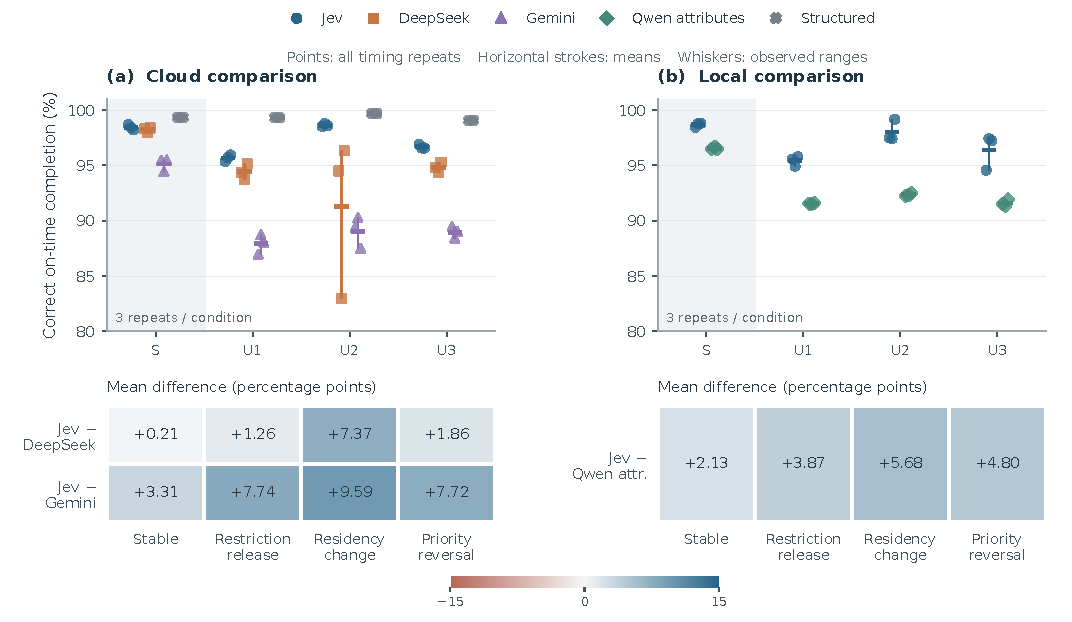
\includegraphics[width=\textwidth]{figures/contract-completion.pdf}
\caption{Correct on-time completion in modeled edge execution. Upper plots show every timing repeat, means (horizontal strokes), and observed ranges (vertical segments). S is stable; U1--U3 are the three update scenarios named below the matrices. Lower cells show Jev-minus-comparator mean differences in percentage points on a common color scale. Each trajectory has 22,500 requests. The local block uses direct-attribute Qwen and its own Jev measurements.}
\label{fig:completion}
\end{figure*}

Across the three update scenarios in the cloud block, mean completion is 97.00\% for Jev, 93.51\% for DeepSeek, and 88.65\% for Gemini. Jev's differences are 3.50 and 8.35 percentage points. Figure~\ref{fig:completion} shows that the size of the difference depends on the transition. Restriction withdrawal, permission replacement, and priority changes alter which placements are useful and which requests have the least remaining slack.

The stable cloud scenario has a much smaller Jev--DeepSeek difference: 98.44\% versus 98.23\%. Both still incur first-use interpretation; subsequent telemetry events reuse the contract. Stable here describes the service requirements: mobility and resource events still occur. The shared scheduler handles that evolving state using the cached contract. The larger updated-condition differences arise when renewed interpretation consumes additional time from the service budget in Eq.~\eqref{eq:remaining-budget}.

The local block shows the same direction with a quality-matched comparator. Mean updated-scenario completion is 96.62\% for Jev and 91.84\% for direct-attribute Qwen, a 4.78-point difference. Stable-condition completion is 98.68\% and 96.55\%, respectively.

\subsection{Completion under Exchanged Waiting Times}
\label{sec:intervention}
To test the timing explanation, we replay each trajectory with the original interpreted contracts and common execution model, exchanging the recorded model waits and numerical scheduling times. The radio events, workload, service rules, and scoring contracts remain fixed. This post-measurement analysis introduces no new model calls.

Let $F(X,C,W)$ denote the completion summary produced by the deterministic execution model. Here $X$ contains the shared radio and workload input, $C$ the sequence of interpreted contracts, and $W$ the recorded model and scheduling durations. For Jev and a comparator, the intervention evaluates $F(X,C_{\mathrm{Jev}},W_{\mathrm{comp}})$ against the comparator's observed modeled summary $F(X,C_{\mathrm{comp}},W_{\mathrm{comp}})$. For the matched-quality pairs, the contract sequences agree. Substituting the comparator's waits tests whether those recorded delays reproduce its service result under the common scheduler.

Each replay set covers four scenarios and three timing repeats; a match requires the full modeled summary to agree. All 12 cloud trajectories exactly reproduce the DeepSeek summaries after this substitution. All 12 local trajectories likewise reproduce direct-attribute Qwen. Thus, the recorded control waits reproduce the modeled completion differences with contract semantics, radio inputs, and scheduling policy held fixed.

\subsection{A Better Local Interface Changes the Baseline}
\label{sec:interface}
\begin{table*}[t]
\centering
\caption{Local interface comparison over 21 calls and 63 contract checks per interface. Completion rates average three stable or nine updated trajectories. Tokens are medians; NC denotes non-comparable token accounting.}
\label{tab:interface}
\footnotesize\setlength{\tabcolsep}{5pt}\renewcommand{\arraystretch}{1.15}
\begin{tabular}{@{}llrrrrrr@{}}\toprule
& & \multicolumn{2}{c}{Interpretation} & \multicolumn{2}{c}{Response (ms)} & \multicolumn{2}{c}{Completion (\%)}\\
\cmidrule(lr){3-4}\cmidrule(lr){5-6}\cmidrule(l){7-8}
\rowcolor{TableHeaderShade}
Model & Interface & Correct & Tokens & Median & [25th, 75th] & Stable & Updated\\\midrule
Jev & Choice & 63/63 & NC & 356.2 & [341.9, 421.2] & 98.68 & 96.62\\
Qwen & Profiles & 33/63 & 28 & 447.9 & [422.1, 466.1] & 87.31 & 85.17\\
Qwen & Attributes & 63/63 & 56 & 757.1 & [750.8, 791.2] & 96.55 & 91.84\\
\bottomrule\end{tabular}\end{table*}

The initial Qwen interface selects identifiers from an 18-profile catalog. It correctly interprets 33 of 63 evaluated contracts. We then change the interface to return location permissions, deadline, and priority directly. The weights, serving instance, business inputs, and non-thinking setting are shared between these two local conditions.

Table~\ref{tab:interface} shows the joint change in quality and time. Direct attribute output reaches 63/63 correct interpretations. Median generated length rises from 28 to 56 tokens, and median response increases from 447.9 to 757.1 ms. Despite the additional waiting, mean updated-scenario completion improves from 85.17\% to 91.84\%. In the restriction-release scenario, the profile interface also produces 2,750 location violations in each timing repeat; these disappear with direct attributes.

The longer attribute response yields better service completion by improving interpretation. It supplies semantic values directly instead of mapping them to catalog identifiers. This interface change combines a different prompt, schema, and output length. Direct-attribute Qwen is consequently the principal local baseline in Sections~\ref{sec:latency}--\ref{sec:intervention} and the application study.

\subsection{Mobile Image Service over NR Access}
\label{sec:application}
\begin{table*}[t]
\centering
\caption{Real image service with simulated NR access. Response cells show median [25th, 75th percentiles] over 16 calls per interpreter. Execution columns retain all 1,080 arrivals per method; exact text is a subset of returned results, and correct on-time completion also imposes contract and deadline requirements. Update windows are fixed 1.5 s intervals after the three updates (180 requests per method). API fees are totals; N/A denotes no billed model API.}
\label{tab:application}
\footnotesize\setlength{\tabcolsep}{5pt}\renewcommand{\arraystretch}{1.15}
\begin{tabular}{@{}lrrrrrrr@{}}\toprule
& \multicolumn{2}{c}{Contract interpretation} & \multicolumn{3}{c}{Execution / 1,080 arrivals} & \multicolumn{1}{c}{Updates} & \multicolumn{1}{c}{Cost}\\
\cmidrule(lr){2-3}\cmidrule(lr){4-6}\cmidrule(lr){7-7}\cmidrule(l){8-8}
\rowcolor{TableHeaderShade}
Method & Correct & Response (ms) & Returned & Exact text & Correct on time & Correct / 180 & API (US\$)\\\midrule
Jev & 48/48 & \shortstack{408.9\\{\scriptsize [341.4, 482.9]}} & 901 & 502 & \shortstack{459\\{\scriptsize (42.50\%)}} & \shortstack{64\\{\scriptsize (35.56\%)}} & 0.001616\\
DeepSeek & 48/48 & \shortstack{497.0\\{\scriptsize [435.1, 566.4]}} & 889 & 498 & \shortstack{463\\{\scriptsize (42.87\%)}} & \shortstack{62\\{\scriptsize (34.44\%)}} & 0.000939\\
Qwen attributes & 48/48 & \shortstack{759.9\\{\scriptsize [754.0, 791.1]}} & 858 & 480 & \shortstack{435\\{\scriptsize (40.28\%)}} & \shortstack{45\\{\scriptsize (25.00\%)}} & N/A\\
Structured & Given & No call & 932 & 510 & \shortstack{473\\{\scriptsize (43.80\%)}} & \shortstack{71\\{\scriptsize (39.44\%)}} & N/A\\
\bottomrule\end{tabular}\end{table*}

The image service preserves the observed semantic quality: Jev, DeepSeek, and direct-attribute Qwen each correctly interpret 48 of 48 contracts across four runs. Their median decision responses are 408.9, 497.0, and 759.9 ms. Jev therefore retains a 17.7\% reduction against DeepSeek and a 46.2\% reduction against Qwen in this application setting.

Table~\ref{tab:application} reports actual correct, on-time image results. Jev completes 459 of 1,080 requests, DeepSeek 463, Qwen 435, and the structured-input reference 473. Jev's full-trajectory result is within four requests, or 0.37 percentage points, of DeepSeek and exceeds Qwen by 24 requests, or 2.22 points. The application therefore retains faster interpretation with similar observed completion to DeepSeek and higher completion than Qwen.

\begin{figure*}[t]
\centering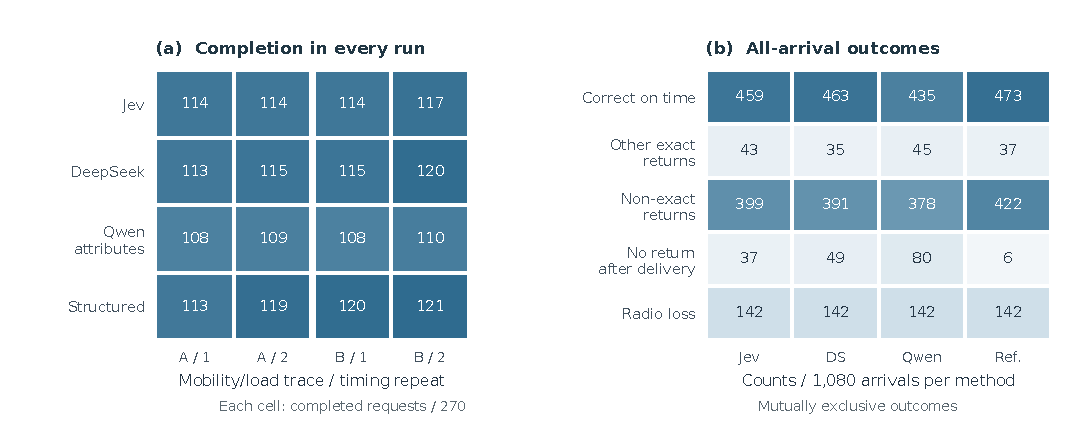
\includegraphics[width=\textwidth]{figures/application-runs.pdf}
\caption{Real image-service execution. (a) Correct on-time counts in all 16 runs, each with 270 arrivals; A and B are the two mobility/load traces, each repeated twice. (b) Mutually exclusive outcomes over all 1,080 arrivals per method. Other exact returns have correct text but fail the full completion criterion; non-exact returns have an incorrect text result. No return after delivery excludes radio losses. DS, Qwen, and Ref. denote DeepSeek, direct-attribute Qwen, and structured input. Color scales run from zero to 125 in (a) and zero to 500 in (b); cell labels give exact counts.}
\label{fig:application}
\end{figure*}

Figure~\ref{fig:application} exposes the per-run comparisons. Jev's differences from DeepSeek are $+1$, $-1$, $-1$, and $-3$ requests; its differences from Qwen are $+6$, $+5$, $+6$, and $+7$. Completion also depends on recognizable text, transfer, and queueing; decision-latency ordering alone does not determine the application outcome.

The fixed update windows contain 180 requests per method. Jev completes 64 correctly and on time, compared with 62 for DeepSeek, 45 for Qwen, and 71 for the structured reference. These windows locate the interval in which fresh interpretation is relevant, while the full-trajectory totals retain the behavior outside updates. The full-run denominator also retains 142 radio-lost images per method. Shared radio delivery makes this loss count identical across interpreters; faster activation benefits delivered requests waiting for a contract. Of the returned results, exact normalized text is obtained for 502 requests with Jev, 498 with DeepSeek, 480 with Qwen, and 510 with the structured reference; the stricter completion counts additionally impose the deadline and contract requirements.

All methods have zero observed location violations in this block. Across the complete matrix, 3,964 foreground and background OCR executions match the service-side records. Every selected image has an actual OCR output, and repeated executions of the same image return consistent text. The completion metric thus counts verified service outputs.
